\documentclass[12pt,a4paper,bibliography=totocnumbered,listof=totocnumbered]{scrartcl}
% u.U. muss Koma-Skript Package ueber MikTeX deinstalliert und neu installiert werden
% Hilft das nicht, so sollte statt scrartcl die Dokumentenklasse article verwendet werden
%\usepackage[backend=bibtex,style=alphabetic]{biblatex}
%\usepackage[backend=bibtex,style=ieee]{biblatex}
\usepackage[style=ieee]{biblatex}
\usepackage[ngerman]{babel}
\usepackage[utf8]{inputenc}
\usepackage{ifthen}
\usepackage{xargs}
\usepackage{amsmath}
\usepackage{amsfonts}
\usepackage{amssymb}
\usepackage{graphicx}
\usepackage{caption}
\usepackage{fancyhdr}
\usepackage{tabularx}
\usepackage{geometry}
\usepackage{setspace}
\usepackage[right]{eurosym}
\usepackage[printonlyused]{acronym}
\usepackage{subfig}
\usepackage{floatflt}
\usepackage[usenames,dvipsnames]{color}
\usepackage{colortbl}
\usepackage{paralist}
\usepackage{array}
\usepackage{titlesec}
\usepackage{parskip}
\usepackage[right]{eurosym}
\usepackage[subfigure,titles]{tocloft}
%\usepackage[pdfpagelabels=true]{hyperref}
\usepackage[pdfpagelabels=true]{hyperref}

\usepackage{listings}
\lstset{basicstyle=\footnotesize, captionpos=b, breaklines=true, showstringspaces=false, tabsize=2, frame=lines, numbers=left, numberstyle=\tiny, xleftmargin=2em, framexleftmargin=2em}
\makeatletter
\def\l@lstlisting#1#2{\@dottedtocline{1}{0em}{1em}{\hspace{1,5em} Lst. #1}{#2}}
\makeatother

%\geometry{a4paper, top=27mm, left=20mm, right=20mm, bottom=35mm, headsep=10mm, footskip=12mm}

\definecolor{javared}{rgb}{0.6,0,0} % for strings
\definecolor{javagreen}{rgb}{0.25,0.5,0.35} % comments
\definecolor{javapurple}{rgb}{0.5,0,0.35} % keywords
\definecolor{javadocblue}{rgb}{0.25,0.35,0.75} % javadoc
\definecolor{gray}{rgb}{0.6,0.6,0.6}
 
\lstset{language=Java,
basicstyle=\ttfamily\footnotesize,
keywordstyle=\color{javapurple}\bfseries,
stringstyle=\color{javared},
commentstyle=\color{javagreen}\itshape\bfseries,
morecomment=[s][\color{javadocblue}]{/**}{*/},
numbers=left,
numberstyle=\tiny\color{gray},
stepnumber=1,
numbersep=10pt,
tabsize=3,
showspaces=false,
showstringspaces=false}
\titlespacing{\section}{0pt}{12pt plus 4pt minus 2pt}{-6pt plus 2pt minus 2pt}

% Kopf- und Fusszeile
\renewcommand{\sectionmark}[1]{\markright{#1}}
\renewcommand{\leftmark}{\rightmark}
\pagestyle{fancy}
\lhead{}
\chead{}
\rhead{\thesection\space\contentsname}
\lfoot{}
\cfoot{}
\rfoot{\ \linebreak Seite \thepage}
\renewcommand{\headrulewidth}{0.4pt}
\renewcommand{\footrulewidth}{0.4pt}

% Vorspann
\renewcommand{\thesection}{\Roman{section}}
\renewcommand{\theHsection}{\Roman{section}}
\pagenumbering{Roman}

\newcommand{\folgen}[1]{
\ensuremath
#1
}

\newcommandx{\student}[3][]{
	\def\studentName{#1}%
	\def\studentMatnr{#2}%
	\def\studentStudiengang{#3}%
}

\newcommandx{\MyTitelseite}[8][]{
\thispagestyle{empty}

\includegraphics[scale=0.2]{pics/oth-logo.png}%\hfill\includegraphics[scale=0.5]{#1}
\begin{center}
\ifthenelse{\equal{#2}{2}}{ % then
	\vspace*{2cm}
	\Large
	\textbf{Ostbayerische Technische Hochschule Regensburg}\\
	\textbf{Fakultät für Informatik und Mathematik}\\
	\vspace*{2cm}
	\Huge
	\textbf{#3}\\[1em]
	\large
	Zur Erlangung des akademischen Grades des\\
	\ifthenelse{\equal{#3}{Bachelorarbeit}}{Bachelor of Science (B.Sc.)}{Master of Science (M.Sc.)}\\
	\vspace*{1cm}
	\Large
	\textbf{#4}\\
}{ % else
	\vspace*{1cm}
	\Large
	\textbf{#4}\\
	\vspace*{2cm}
	\large
	An der Fakultät für Informatik und Mathematik der\\
	Ostbayerischen Technischen Hochschule Regensburg\\
	im Studiengang\\
	\studentStudiengang\\[2em]
	eingereichte\\
	\vspace*{1cm}
	\Large
	\textbf{#3}\\[2em]
	\large
	zur Erlangung des akademischen Grades des\\
	\ifthenelse{\equal{#3}{Bachelorarbeit}}{Bachelor of Science (B.Sc.)}{Master of Science (M.Sc.)}
	\vspace*{1cm}
	\Large
}
	\vfill
	\normalsize
	%\newcolumntype{x}[1]{>{\raggedleft\arraybackslash\hspace{0pt}}p{#1}}
	\begin{tabular}{rl}%{6cm}p{7.5cm}}
	    \rule{0mm}{1ex}\textbf{Vorgelegt von:} & \studentName \\
		\rule{0mm}{1ex}\textbf{Matrikelnummer:} & \hspace*{-0.5em}\begin{tabular}[t]{r}\studentMatnr\end{tabular} \\ 
		\ifthenelse{\equal{#2}{1}}{~\\}{\rule{0mm}{1ex}\textbf{Studiengang:} & \studentStudiengang \\[2em]}
		\rule{0mm}{1ex}\textbf{Erstgutachter:} & #5 \\ 
		\rule{0mm}{1ex}\textbf{Zweitgutachter:} & #6 \\[2em]
		\rule{0mm}{1ex}\textbf{Abgabedatum:} & #7 \\ 
	\end{tabular} 
\end{center}
\pagebreak
}
%\addbibresource{literatur.bib}
\addbibresource{mendeley_v2.bib}


\begin{document}


% ----------------------------------------------------------------------------------------------------------
% Titelseite
% ----------------------------------------------------------------------------------------------------------
\newcommand{\studierenderName}{Philipp Gottschalk}
\student{\studierenderName}		% Studierender
{2853044}						% Matrikelnummer
{Technische Informatik}			% Studiengang

\MyTitelseite{}	% Optionales Logo des extern betreuenden Unternehmens
{1}								% Style der Titelseite (1 oder 2)
{Bachelorarbeit}				% Typ der Abschlussarbeit (\in {Bachelorarbeit, Masterarbeit})
{Analyse und Vergleich von Prozess-Isolationsmechanismen bei Containern und Virtuellen Maschinen}				% Thema der Arbeit						
{Prof.\ Dr.\ Alexander Metzner}		% Betreuer
{Prof.\ Dr.\ Richard Roth}	% Zweitgutachter
{13.10.\the\year}				% Abgabedatum


\thispagestyle{empty}
~\pagebreak

\setcounter{page}{1} 

% ----------------------------------------------------------------------------------------------------------
% Eigensctändigkeitserklaerung
% ----------------------------------------------------------------------------------------------------------
\thispagestyle{empty}
\section*{Erklärung zur Bachelorarbeit}

\bigskip
\bigskip 
\bigskip 

\begin{enumerate}
    \item Mir ist bekannt, dass dieses Exemplar der Bachelorarbeit als Prüfungsleistung in das Eigentum der Ostbayerischen Technischen Hochschule Regensburg übergeht.
    \item Ich erkläre hiermit, dass ich diese Bachelorarbeit selbständig verfasst, noch nicht anderweitig für Prüfungszwecke vorgelegt, keine anderen als die angegebenen Quellen und Hilfsmittel benutzt sowie wörtliche und sinngemäße Zitate als solche gekennzeichnet habe.
\end{enumerate}

\bigskip 
\bigskip 
\bigskip 

Regensburg, den \today

\bigskip 
\bigskip

\line(1,0){200}
\newline
\studierenderName

% ----------------------------------------------------------------------------------------------------------
% Abstract
% ----------------------------------------------------------------------------------------------------------
\thispagestyle{empty}
\setstretch{1.15} % Zeilenspacing
\section*{Zusammenfassung}

\bigskip 


In der folgenden Arbeit wird $\ldots$


% ----------------------------------------------------------------------------------------------------------
% Inhaltsverzeichnis
% ----------------------------------------------------------------------------------------------------------
\tableofcontents
\pagebreak

% ----------------------------------------------------------------------------------------------------------
% Abbildungsverzeichnis
% ----------------------------------------------------------------------------------------------------------
\lhead{}
\rhead{Abbildungsverzeichnis}
\listoffigures
\pagebreak

% ----------------------------------------------------------------------------------------------------------
% Tabellenverzeichnis (optional)
% ----------------------------------------------------------------------------------------------------------
\lhead{}
\rhead{Tabellenverzeichnis}
\listoftables
\pagebreak

% ----------------------------------------------------------------------------------------------------------
% Listingsverzeichnis (optional; Code nur, wenn wirklich sinnvoll und wichtig)
% ----------------------------------------------------------------------------------------------------------
%\lhead{}
%\rhead{Quellcodeverzeichnis}
%\lstlistoflistings
%\pagebreak

% ----------------------------------------------------------------------------------------------------------
% Abkürzungsverzeichnis (optional)
% ----------------------------------------------------------------------------------------------------------
\lhead{}
\rhead{Abkürzungsverzeichnis}
%\listoftables
\section{Abkürzungsverzeichnis}
\begin{acronym}[KDE]
\acro{BA}[BA]{Bachelorarbeit}
\acro{MA}[MA]{Masterarbeit}
\end{acronym}
\pagebreak


% ----------------------------------------------------------------------------------------------------------
% Inhalt
% ----------------------------------------------------------------------------------------------------------
% Abstände Überschrift
\titlespacing{\section}{0pt}{12pt plus 4pt minus 2pt}{0pt plus 2pt minus 2pt}
\titlespacing{\subsection}{0pt}{12pt plus 4pt minus 2pt}{0pt plus 2pt minus 2pt}
\titlespacing{\subsubsection}{0pt}{12pt plus 4pt minus 2pt}{0pt plus 2pt minus 2pt}
%\titlespacing{\Paragraph}{0pt}{12pt plus 4pt minus 2pt}{0pt plus 2pt minus 2pt}
% Kopfzeile
\renewcommand{\sectionmark}[1]{\markright{#1}}
\renewcommand{\subsectionmark}[1]{}
\renewcommand{\subsubsectionmark}[1]{}
%\renewcommand{\paragraphmark}[1]{}

\lhead{Kapitel \thesection}
\rhead{\rightmark}

%\onehalfspacing
\setstretch{1.15}
\renewcommand{\thesection}{\arabic{section}}
\renewcommand{\theHsection}{\arabic{section}}
\setcounter{section}{0}
\pagenumbering{arabic}
\setcounter{page}{1}

\setcounter{secnumdepth}{4}
\titleformat{\paragraph}
{\normalfont\normalsize\bfseries}{\theparagraph}{1em}{}
\titlespacing*{\paragraph}
{0pt}{3.25ex plus 1ex minus .2ex}{1.5ex plus .2ex}

% ----------------------------------------------------------------------------------
% Kapitel: Einleitung
% ----------------------------------------------------------------------------------


%\thispagestyle{empty}
\section{Einleitung}
In der Industrie geht es meist darum wie man Kosten einsparen kann. Die Hardware Systeme in Firmen werden häufig nur zu einem geringen Prozentsatz ausgelastet. Neue Hardware für zusätzliche Anforderungen ist sehr teuer. Wenn es nur eine Möglichkeit geben würde auf einem System mehrere voneinander Isolierte Umgebungen zu schaffen und die schon vorhandenen Kapazitäten auszunutzen, könnten kosten durch neue Anschaffung, Platz und sogar Strom gespart werden. Vorallem in der Automobilindustrie geht es bei der Entwicklung von Serienfahrzeugen um möglichst effizient ausgenutzte Räume und Ressourcen. Bereits Cent Beträge die Pro Fahrzeug eingespart werden können, schlagen bei einer Millionenfachen Produktion zu Buche. 

Container als leiftgewichtiger Virtualierung bietet ein 

gegenüberstellung Effizienz Isolierung 
Hardwareaufwand
Ausfallsicherheit 

\subsection{Motivation}
\subsection{Projektbeschreibung}
\subsection{Ziele}

Effiziente ressourcenverteilung 

Überlastung der Hardware
geld sparen 




\pagebreak


% ----------------------------------------------------------------------------------
% Kapitel: Theorie
% ----------------------------------------------------------------------------------

\thispagestyle{empty}
\subsection{Kernel}

\section{Theorie}
\subsection{Container}
Container-basierte Virtualisierung ist ein leichtgewichtiger Virtualisierungsansatz auf Betriebssystemebene, bei dem der Host-Kernel zur Ausführung mehrerer virtueller Umgebungen verwendet wird. Diese virtuellen Umgebungen werden oft einfach als \glqq Container \grqq{} bezeichnet. Linux-V Server[X], Open VZ\cite{IndexOpenvz.org} und Linux Container(LXC)\cite{IndexLinuxcontainers.Org} sind die drei wichtigsten Vertreter dieses Ansatzes. Die allgemeine Architektur einer Container-basierten Virtualisierungslösung ist in (Abb \ref{fig:architecture}) dargestellt. Containerbasierte Virtualisierung erfolgt auf Betriebssystem Ebene, so dass mehrere Anwendungen ohne redundante Ausführung anderer Betriebssysteme auf dem Host betrieben werden können. Container sehen von außen aus wie normale Prozesse, die auf dem Kernel laufen, der mit dem Host-Rechner geteilt wird. Sie stellen eine isolierte Umgebung mit den notwendigen Ressourcen für die Ausführung von Anwendungen zur Verfügung. Diese Ressourcen können entweder mit dem Host geteilt oder separat im Container installiert werden \cite{Xavier2014AClusters}. Namespaces sind die Basis des LXC und stellen in Verbindung mit anderen Ressourcen-Management-Systemen eine isolierte Umgebung in Form von Containern zu Verfügung. LXC nimmt die cgroups Ressourcenverwaltungseinrichtungen\cite{Heo2015ControlV2} als Grundlage und fügt POSIX file Fähigkeiten [X] hinzu, um die Ressourcen unter den Containern einzuschränken. 

\vspace{1em}
\begin{minipage}{\linewidth}
	\centering
	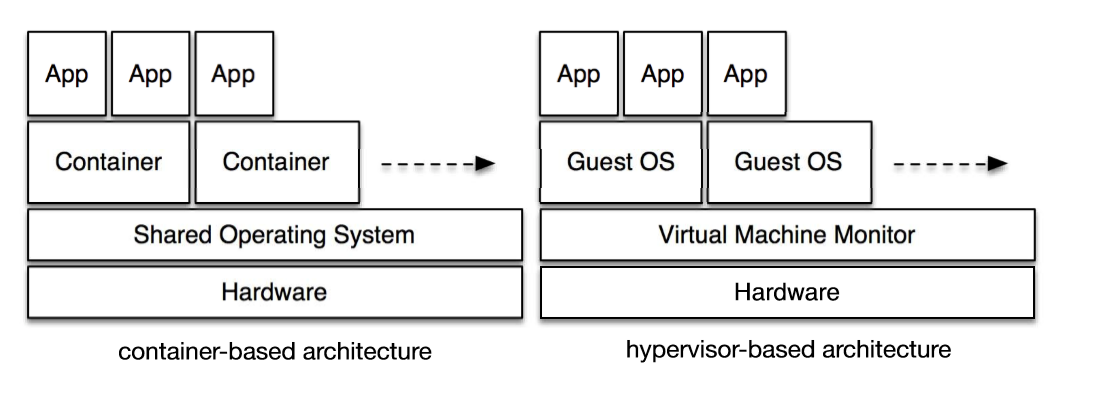
\includegraphics[width=1\linewidth]{pics/docker2.png}
	\captionof{figure}[Architektur]{Aufbau Container und Virtuelle Maschine \cite{Xavier2015AClouds}}
	\label{fig:architecture}
\end{minipage}


\subsection{Virtuelle Maschine}
Eine Virtuelle Maschine Bildet mit Hilfe des Virtuellen Maschinen Monitors (VMM)/Hypervisor eine komplette Rechnerarchitektur auf dem Host-Rechner nach (siehe Abb \ref{fig:architecture}). Man unterscheidet zwischen zwei Arten von VMM: Dem Typ 1 VMM oder "Bare-Metal-Hypervisor" genannt, welcher direkt auf der zugrundeliegenden Hardware des Hosts liegt und dem Typ-2-VMM "gehosteter Hypervisor" welcher eine komplette virtuelle Maschine auf dem Host Betriebssystem erstellt (siehe Abb \ref{fig:Hypervisor_Typ1/Typ2}).

\vspace{1em}
\begin{minipage}{\linewidth}
	\centering
	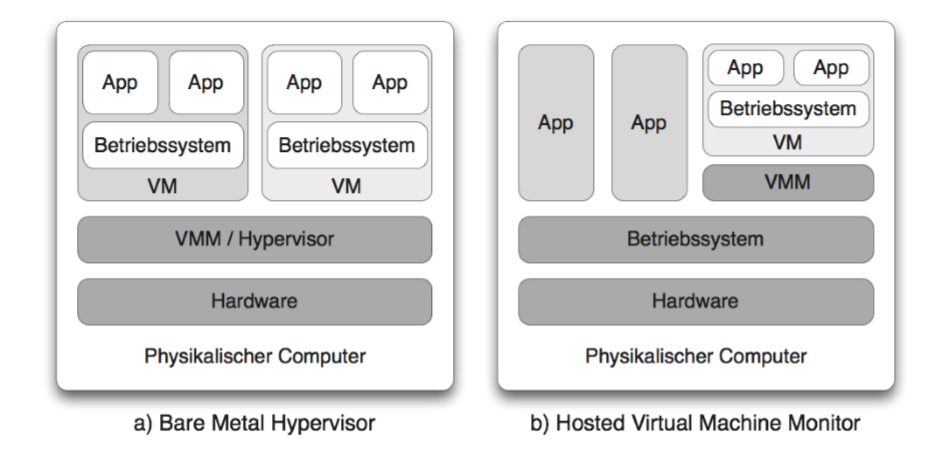
\includegraphics[width=1\linewidth]{pics/Hypervisoren.PNG}
	\captionof{figure}[Hypervisor Typ1/Type2]{Hypervisor Typ1/Typ2 \cite{Meinel2011VirtualisierungMarktubersicht} }
	\label{fig:Hypervisor_Typ1/Typ2}
\end{minipage}

\subsubsection{Typ-1-VMM}
Der VMM kümmert sich um die Ressourcenverwaltung und die Bereitstellung von Virtuellen Maschinen und stellt ein eigenes Betriebssystem dar. Die Aufteilung der Rechenzeit und die Zuteilung von Speicher auf die einzelnen VMs sind beispiele der Aufgaben welche die Ressourcenverwaltung übernimmt.VMware ESX [X] ist ein Beispiel für diesen Virtuallisierungs Ansatz, das mit einem eigenen Treiber nur direkt auf der Hardware laufen kann.

\subsubsection{Typ-2-VMM}
Ein Typ-2-VMM teilt sich ein Gastgeberbetriebssystem(Host) mit anderen Applikationen. Um die nötigen Rechte auf der Hardware zu erhallten, wird ein spezieller VMM-Treiber verwendet, der direkt unter dem Host-system installiert wird. Dieser ermöglicht Privilegierte Zugriffsrechte auf den Kern.

Ganz gleich, welche Methode der Virtualisierung zum Einstz kommt, eins haben sie gemeinsam: Einige Befehle, die das Gastsystem an die CPU sendet, müssen über die Virtualisierungsschicht abgefangen und interpretiert werden \cite{Glatz2015Betriebssysteme}.




\subsection{Isolation}
Das Ziel der Prozessisolation ist es, zu verhindern, dass Container untereinander beeinflussbar sind. Dieses Unterfangen ist mit Hilfe der sogenannten "namespaces" möglich. Die Ressourcen Isolation gewährleistet, dass Prozesse nur einen zugeteiltet anteil einer verfügbaren Ressource verwenden können, dies gelingt mit Hilfe der Cgroups.

\subsubsection{Namespaces drüberschauen buch seite 68}
Seit der Einführung der Kernel Namespaces ist es möglich, Ressourcen des Kernsystems  voneinander zu isolieren und diese Teile unter bestimmten Voraussetzungen anderen Anwendungen/Prozessen zur Verfügung zu stellen. 

Wenn man sich die zugrunde liegenden Funktionsaufrufe anschaut erkennt man, dass fast alle Namespaces via clone- und stnsOperationen zur Verfügung gestellt werden. Für den oder die Prozesse innerhalb eines Namespaces ist dies jedoch nicht erkennbar. Der innerhalb eines Namespaces gestatete Prozessaufruf arbeitet isoliert und sieht nur sich selbst und seine Kindprozesse, jedoch nicht die übergeordnete Umgebung, während der übergeordnete Prozess natürlich alle Namespaces und darin laufende Prozesse sieht. 

Derzeit existieren sechs verschiedene Namensräume, unter anderem der PID Namespace. Er kann uns über die Namespace-Abschottung z.B. einen sogenannten nested Process Tree zur Verfügung stellen, also einen gekapselten Prozessbaum innerhalb des eigentlichen (Host-)Prozessbaumes, in welchem unsere Container-Instanz läuft. Aber dies ist nicht der einzige Namspace, an dem unsere Container partizipieren dürfen.

Die vereinfachte Darstellung des PID Namespaces einer gespawnten bzw geforkten Container-Prozess-Umgebung ist in Abbildung \ref{fig:PID} dargestellt. \cite{Liebel2017SkalierbareContainer-Infrastrukturen}

\vspace{1em}
\begin{minipage}{\linewidth}
	\centering
	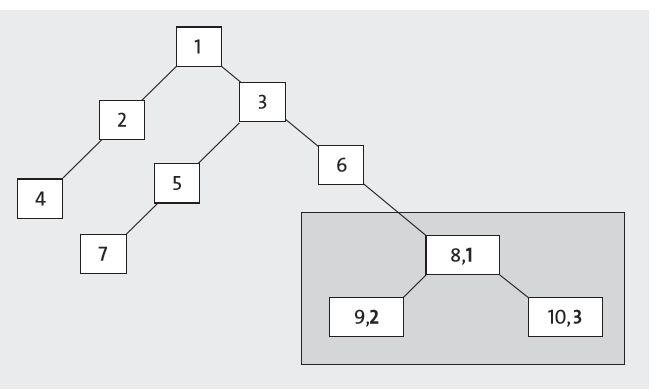
\includegraphics[width=1\linewidth]{pics/PID.PNG}
	\captionof{figure}[PID]{ PID Namespaces für Host und Container (im Fettdruck) \cite{Liebel2017SkalierbareContainer-Infrastrukturen}}
	\label{fig:PID}
\end{minipage}

\subparagraph{PID-Namespace} ist hierarchisch[X] deshalb kann ein Prozess nur die anderen Prozesse in seinem eigenen Namensraum oder in seinen untergeordneten Namensräumen sehen. Folglich kann der Host die Prozesse innerhalb des neuen PID-namespace des Containers beobachten und beeinflussen, aber die Prozesse innerhalb des Containers können die anderen Prozesse, die im Host oder in anderen Containern laufen, nicht beobachten oder beeinflussen

\subparagraph{Mount-Namespace} isoliert filesystem Mountpunkte, die von einem Container gesehen werden, so dass Prozesse in verschiedenen Containern unterschiedliche Ansichten der file Systemhierarchie haben können.

\subparagraph{UTS-Namespace} erlaubt es jedem Container seinen eigenen Hostnamen und NIS-Domänennamen zu haben.

\subparagraph{IPC-Namespace} isoliert die Interprozesskommunikation, das bedeutet Prozesse, die in einem Container enthalten sind, haben eigene Nachrichten Warteschlangen und sind völlig unabhängig von Prozessen in anderen Containern.

\subparagraph{Network namespace} isoliert das Netzwerk-Untersystem wie z.B. Geräte und IP-Adressen. Jeder Container unterhält seine eigene Netzwerk Konfiguration und die darauf laufenden Anwendung.

\subparagraph{User-Namespace} isoliert Benutzer-IDs vom Host und anderen laufenden Containern. Das bedeutet, dass der Benutzer root (ID0) innerhalb eines Containers volle Privilegien hat, aber keine Privilegien außerhalb, was Sicherheit und Zuverlässigkeit gewährleistet. \cite{Xavier2015AClouds}
	



\subsubsection{cgroup}
\glqq c-group\grqq{} steht für \glqq contol group\grqq{}. Durch cgroup ist es möglich, eine Reihe von Kriterien anzuwenden, um Ressourcen wie Speicher,Netzwerk, Festplatten-I/O und CPU einzuschränken. Ein Container sollte seine auferlegten Beschränkungen nicht überschreiten und andere Container, die auf derselben Hardware laufen, nicht stören. Cgroup ist für die Ressourcen Begrenzung, Priorisierung, Abrechnung und Kontrolle zuständig.\cite{Heo2015ControlV2} 

cgroup ist ein Mechanismus, um Prozesse und System Ressourcen entlang der Hierarchie in einer kontrollierten und konfigurierbaren weise hierarchisch zu organisieren. cgroup besteht im Wesentlichen aus zwei Teilen, dem Kern und dem Controller. Der cgroup Kern ist in erster Linie für die hierarchische Organisation von Prozessen zuständig. Der cgroup Controller ist in der Regel für die Verteilung einer bestimmten Art von System Ressource entlang der Hierarchie verantwortlich. Cgroup bilden eine Baumstruktur und jeder Prozess im System gehört genau zu einer cgroup. Alle Unterprozesse (Kind Prozesse) eines Prozesses (Eltern Prozess) gehören zur gleichen cgroup. Alle neu erstellten Prozesse gehören zu der cgroup zu der auch der Eltern Prozess gehört.


\paragraph{Ressourcen Verteilungs Modelle}
Cgroup Controller verfügen über verschiedene Ressourcen Verteilungs Modelle. Die Modelle sind auf die Art und den Verwendungszweck der Ressource zugeschnitten. Dieser Paragraph befasst sich mit den verschiedenen Hauptschemen und deren Aufgaben.

----CPU kann kein Prozent wert zugeteilt werden weil durch eine geringe Auslastung die Leistung runter fährt (youtube video siehe one noteJérôme Petazzoni )

\subparagraph{Weight}
Die Ressourcen eines Prozesses werden Proportional an alle aktiven Kind Prozesse verteilt. Da nur die aktiven Kind Prozesse welche aktuell Ressourcen benötigen an der Verteilung teilnehmen, werden die zugeteilten Ressourcen effizient genutzt. 

Alle Konfigurationen sind gültig und es gibt keinen Grund, Migrationen von Konfigurationsänderungsprozessen abzulehnen.

\subparagraph{Limit}
Ist ein High-Limit gesetzt, kann ein Kind Prozess nur bis zu der konfigurierten Menge einer Ressource Verwenden. Low/High Limits können auch als soft-Limits bezeichnet werden. Die Summe der Limits aller Kind Prozesse kann die zur Verfügung stehende Menge an Ressourcen des Eltern Prozesses überschreiten. Ein Limit ist sozusagen ein maximaler Richtwert der bei dringendem Bedarf überschritten werden kann. Der Prozess welcher den über das Limit hinaus ragende Anteil verwendet, steht unter erhöhtem Druck und wird gedrängt die Ressource schnell wieder frei zu geben. Wenn eine cgroup die Ressourcen nicht mehr benötigt, wird diese bis zu einem setzbaren Low-Limit freigegeben.

Da Limits überschritten werden können, sind alle Konfigurationen gültig und es gibt keinen Grund Konfigurationsänderungen zurück zu weisen.

\subparagraph{Protection}
Eine cgroup ist so geschützt, dass sie bis zur konfigurierten Menge der Ressource fest zugeordnet werden kann, wenn die Verwendung aller Prozesse unter der geschützten Ebene Liegt. Der Schutz kann garantiert oder effizient sein. Bei garantiertem Schutz wird die Ressource explizit für die cgroup frei gehalten und kann vollständig verwendet werden. Die Effizientere Variante bietet die Möglichkeit zugeteilte Ressourcen auf Anfrage für andere Prozesse frei zu stellen.

Die Protectionen können überschritten werden somit sind alle Konfigurationsmethoden gültig.

\subparagraph{Allocation}
Einer cgroup wird eine bestimmte Menge einer Ressource fest zugeteilt und stellt somit ein Hard-Limit dar. Die Summe der Zuweisungen von Kind Prozessen dürfen die Menge der fest zugeteilten Ressource des Eltern Prozesses nicht überschreiten. Auch wenn die Ressource nicht ausgenutzt wird, bleibt diese der cgroup erhalten. 

Es gibt bei Allocationen einige Konfigurationen die zurückgewiesen werden. Wenn bei der Bildung eines neuen Prozesses die zur Ausführung benötige Ressourcenmenge überschritten werden, wird der Prozess verworfen.

\paragraph{Ressourcen Modellierung}
Im folgenden Paragraphen werden Art der Ressource mit verwendetem Modell aufgelistet

\subparagraph{Speicher}
Der Speicher Controller regelt die Verteilung des Speichers. Speicher ist zustandsabhängig und verwendet sowohl Limit als auch Protection Modelle. Aufgrund der Verflechtung zwischen Speicherbedarf und Speicherrückgabeforderung ist die Verwaltung sehr kompliziert.

Memory-low(Best-effort)
Der geforderte Mindestanteil wird gestellt. Unbenutzer Speicher kann bei Bedarf vom System verwendet werden.

Memory-High(Best-effort)
Dies ist der Hauptmechanismus zur Steuerung des Speicherverbrauchs einer cgroup. WEnn die Nutzung einer cgroup über die obere Grenze hinausgeht, werden die Prozesse der cgroup gedrosselt und unter starken Reklamationsdruck gesetzt.

Memory-min(Hard-Limit)
Falls der Speicherverbrauch einer cgroup innerhalb seiner effektiven minimalen Grenze liegt, wird der Speicher der cgroup unter keinen Umständen zurückgefordert. Wenn nicht genug Speicherplatz zur Verfügung steht um die Minimalanforderung zu gewährleisten, kommt der OOM-Killer zum Einsatz und schafft freien Speicher.

Memory-max(Hard-Limit)
Wenn der Speicherverbrauch einer cgroup diese Grenze erreicht und nicht reduziert werden kann, wird der OOM-Killer in der cgroup aufgerufen, dies ist der letzte Schutzmechanismus. Unter bestimmten Umständen kann ein Prozess vorübergehend über das Limit hinaus gehen.

\subparagraph{CPU}
Der CPU Controller reguliert die Verteilung der CPU-Zyklen. Diese Steuerung Verwendet Gewichtung und Limit Modelle für normale Ressourcen Verteilung und das Allocation Modell für eine Echtzeit Verteilung.

Die CPU kann nicht auf einen genauen gleichbleibenden Prozentwert angegeben werden, da sich die Leistung der CPU aus Energie Effizienz gründen an die Auslastung anpasst.

\subparagraph{IO}
Der IO Controller reguliert die Verteilung der IO Ressourcen. Der Controller verwendet Gewichtung und Limit Modelle. Die Gewichtung gibt die relative IO-Zeit and, die die cgroup in Bezug auf ihre Geschwister verwenden kann.



\paragraph{OOM-Killer}



\subsubsection{Sicherheit-Container / Umschreiben!}
In den letzten Jahren unterlag die Entwicklung von Container-Systemen wie Docker, Rocket und andern einer sehr schnellen Evolution. Dabei war der Fortschritt der Technologie wichtiger als die Sicherheit hinter dem System. Es existieren zahlreiche Studien, die alle auf den Schluss kommen, dass viel Potential in der Entwickelten Technologie steckt, doch die Sicherheit noch nicht ausreichend gegeben ist.

Zwei Punkte spielen eine große Rolle. Zum einen die Sicherheit und Vertrauenswürdigkeit der Images, die den Container-Instanzen zugrunde liegen, zum anderen die oben benannten Namespaces. Die Nutzung von Namespaces stellt einen direkten Zugriff auf den Host-Kernel dar, ein Bereich zu dem sich Angreifer bei anderen Systemen erst einmal mühevoll durchkämpfen müssen.



%\pagebreak

 ----------------------------------------------------------------------------------
% Kapitel: Praktische Umsetzung
% ----------------------------------------------------------------------------------

%\thispagestyle{empty}
\section{Praktische Durchführung}
\subsection{Hardware}
\subsection{Docker}
\subsection{Realisierung}
Im Linux-File-System ist es möglich cgroups über PID's ausfindig zu machen und die verwendeten Ressourcen auszugeben. Was zu der Idee führte, einen neuen Docker-Container zu erstellen, in diesem einen Prozess mit einem einfachen malloc() befehlt in einer Endlosschleife auszuführen und die menge des allokierten Speichers der cgroup auszuwerten. 

\subparagraph{Test01}
Über das online user interface war es möglich einen Docker-Container zu erstellen. Ressourcen Limits konnten ebenfalls vor dem starten des Containers eingestellt werden. Für den ersten Start des Containers sind allerdings noch keine Begrenzungen des Speichers nötig, da es in erster Linie um die Auswirkung des ausgeführten C-Programms auf die eigene cgroup geht. Der verwendete C-Code den der Prozess ausführen wird, ist in Listing \ref{01mem} zu sehen. Ein erstelltes Skript verwendet die beim Start erzeugte PID, findet die Cgroup in der der Prozess ausgeführt wird und schreibt die ausgelesenen Messdaten in ein txt-File. Die Messdaten wie Clock-Time in Nanosekunden und Speicherverbrauch in Bytes werden für die Auswertung verwendet.

\vspace{1em}
\lstinputlisting[caption=einfacher C-Code, label=01mem, basicstyle=\ttfamily\scriptsize]{code/01mem.txt}

\subparagraph{Erwartungshaltung Test 01}
Falls das Skript die Messwerte in ungefähr gleichmäßig schnellen Abständen liefert, und die Speicher Allocationen gleich schnell ablaufen, wird eine Gerade Funktion hypothetisch erwartet, die gleichbleibend schnell ansteigt und irgendwann wenn nicht mehr genug Speicher im System vorhanden ist beendet wird.

\vspace{1em}
\begin{minipage}{\linewidth}
	\centering
	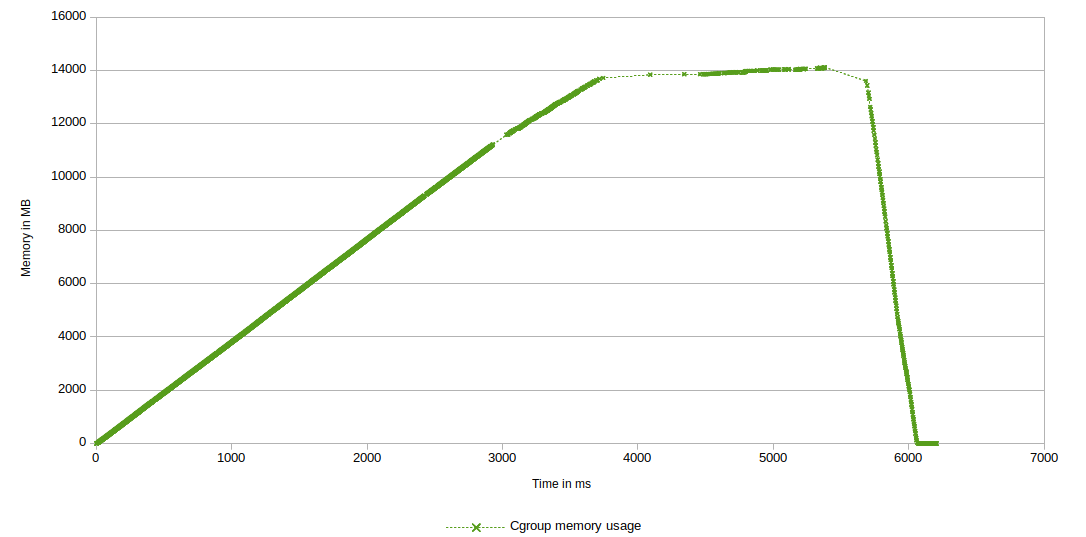
\includegraphics[width=1\linewidth]{pics/001_mem_usage_No_Limit_Cgroup_RDY_FOR_USE.png}
	\captionof{figure}[Speicher Verbrauch Cgroup Ohne Limit]{Memory usage Cgroup no Limit}
	\label{fig:001_mem_usage_No_Limit_Cgroup_RDY_FOR_USE}
\end{minipage}

\subparagraph{Ergebnis Test01}
In Abbildung \ref{fig:001_mem_usage_No_Limit_Cgroup_RDY_FOR_USE} ist wie erwartet eine gleichmäßige Steigung erkennbar. Bei ca. 13900MB Allociertem Speicher bricht die Wachstumsrate zusammen. An diesem Punkt ist der insgesamt 16GB große Arbeitsspeicher größtenteils Ausgeschöpft. Ein paar MegaByte konnten vom Betriebssystem für den dauerhaft nach mehr Speicher verlangendem Prozess bereitgestellt werden. Bei knapp über 14000MB wurde der OOM-Killer eingeschaltet um wichtigere Prozesse zu schützen, und der Container wurde beendet.

\subparagraph{Test02}
Im nächsten Schritt wird der Verlauf einer Cgroup näher betrachtet, bei der ein Speicherlimit festlegt wird, das nicht überschritten werden soll (Hard-Limit). Um dieses Limit zu erstellen, wird im User-Interface  das Ressourcenlimit auf 8200 Megabyte gesetzt und das in Listing \ref{01mem} vorgestellte Programm nochmals ausgeführt.

\subparagraph{Erwartungshaltung Test 02}
Da nun ein Hard-Limit eingerichtet ist wird prognostiziert, dass die Cgroup mit der gleichen Geschwindigkeit wie in Abbildung \ref{fig:001_mem_usage_No_Limit_Cgroup_RDY_FOR_USE} bis zum gesetzten Limit ansteigt und dieses nicht überschreiten wird. 

\vspace{1em}
\begin{minipage}{\linewidth}
	\centering
	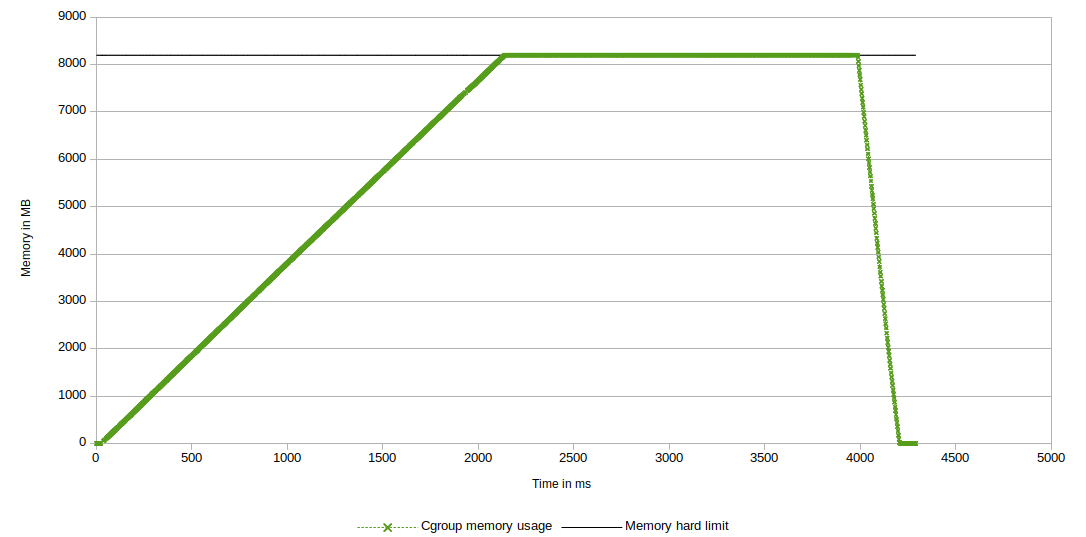
\includegraphics[width=1\linewidth]{pics/002_mem_usage_8200mb_limit_Cgroup_RDY_FOR_USE.png}
	\captionof{figure}[Speicher Verbrauch Cgroup 8200MB Limit]{Memory usage Cgroup 8200MB Limit}
	\label{fig:002_mem_usage_8200mb_limit_Cgroup_RDY_FOR_USE}
\end{minipage}

\subparagraph{Ergebnis Test02}
Mit einer Allocations Rate von ca. 4000MB/S auf dem ausgeführten Host-System ändert sich an der Speicher Zugriffsrate nichts, das Limit von 8200MB wurde erfolgreich eingehalten und der Prozess wurde wieder vom Betriebssystem beendet.

Schon fast Vorbildlich hält sich die Cgroup an das gesetzte Limit. Da stellt sich die Frage "wie kann man sich eine Cgroup anschaulich vorstellen, was zeigt sie an, wie weit kann sie verwendete Ressourcen der einzelnen Prozesse verfolgen?". 


Die Cgroup ist wie eine Box. Die Größe der Box wird bei der Erstellung des Containers festgelegt. In Abbildung \ref{fig:002_mem_usage_8200mb_limit_Cgroup_RDY_FOR_USE} waren es 8200MB. Der Füllstand der Box setzt sich aus den verwendeten Ressourcen aller in der Box ausgeführten Prozesse zusammen. Wenn ein Prozess nun wie in Abbildung \ref{fig:002_mem_usage_8200mb_limit_Cgroup_RDY_FOR_USE} die Komplette Box ausfüllt und weiter darüber hinaus ragen würde, wäre die Box nur in der Lage den Füllstand bis zu Ihrer Maximalgröße von 8200 MB wiederzuspiegeln. Der Überlaufende teil des Prozesses kann von der Cgroup nicht erkannt werden.

\subparagraph{Test03}
Nach dem Einblick der Anzeigemöglichkeiten einer Cgroup liegt es nun nahe, den Prozess der durch das Ausführen des oben genannten C-Codes entsteht, genauer anzusehen. Der Test02 wird mit einer Skript Erweiterung um die Anzahl der verwendeten Memory-Pages des Prozesses wiederholt. Eine Memory-Page ist 4KB groß und wird für die Auswertung mit der Anzahl an Memory-Pages multipliziert.

\subparagraph{Erwartungshaltung Test 03}
Wenn die Memory-Page Größe multipliziert mit der Anzahl an verwendeten Memory-Pages genau dem entspricht, was die Cgroup an Speicher Allocation ausgibt, sollten beide Graphen bis zum erreichen des Limits parallel verlaufen.

\vspace{1em}
\begin{minipage}{\linewidth}
	\centering
	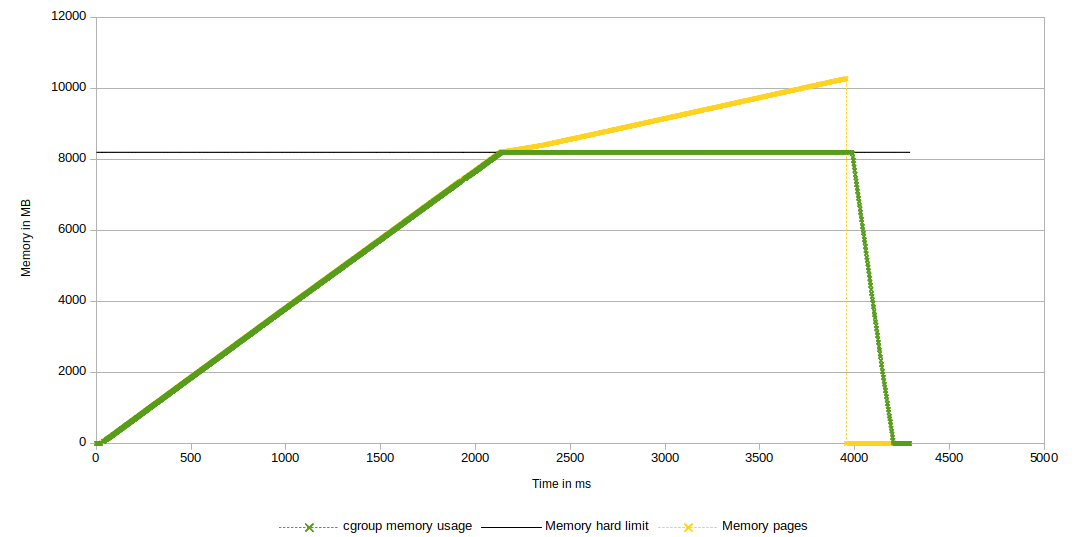
\includegraphics[width=1\linewidth]{pics/003_mem_usage_8200mb_limit_Cgroup_Pages_RDY_FOR_USE.png}
	\captionof{figure}[Speicher Verbrauch Cgroup 8200MB Limit]{Memory usage Cgroup 8200MB Limit}
	\label{fig:003_mem_usage_8200mb_limit_Cgroup_Pages_RDY_FOR_USE}
\end{minipage}

\subparagraph{Ergebnis Test03}
Deutlich zu erkennen sind die exat aufeinanderliegeneden Messwerte der Cgroup und der Memory Pages. Ab 8200MB schießen die allocierten Memory Pages bis ca 10200MB über das Limit hinaus. Erkennbar ist auch die geringere Allocationsrate sofort nach dem Überlauf auf 2000MB/s fällt. Komplett ignoriert wurde das Limit allerdings nicht. Verglichen mit Abbildung \ref{fig:001_mem_usage_No_Limit_Cgroup_RDY_FOR_USE} war noch genügend Speicher im System vorhanden. Wieso wurde der Prozess dann überhaupt schon beendet, warum konnte er über das Limit hinaus allokieren, wie verhält sich ein Container wenn er nur ein wenig über das Limit geht, wie wirkt sich das auf andere Container im System aus?

\subparagraph{Test04}
Um auf die aufgekommenen Fragen in Paragraph "Ergebnis Test03" hin zu arbeiten, benötigen wird nun ein Container der für eine gewisse Zeitspanne läuft und etwas mehr als das gesetzte Limit allociert benötigt. Der in Listing \ref{01mem} gezeigte C-Code wurde zu Listing \ref{02mem} verändert. 

\vspace{1em}
\lstinputlisting[caption=einfacher C-Code, label=02mem, basicstyle=\ttfamily\scriptsize]{code/02mem.txt}

\subparagraph{Erwartungshaltung Test 04}
Nachdem der Malloc(sizeof(int)*1024) befehl nun 2200001 mal ausgeführt wird, ein Integer 4Byte groß ist *1024 sind 4KB pro Ausführung, sollte der Graph der Memory Pages bei etwa 8600MB verharren und 60 Sekunden diesen Wert halten.

\vspace{1em}
\begin{minipage}{\linewidth}
	\centering
	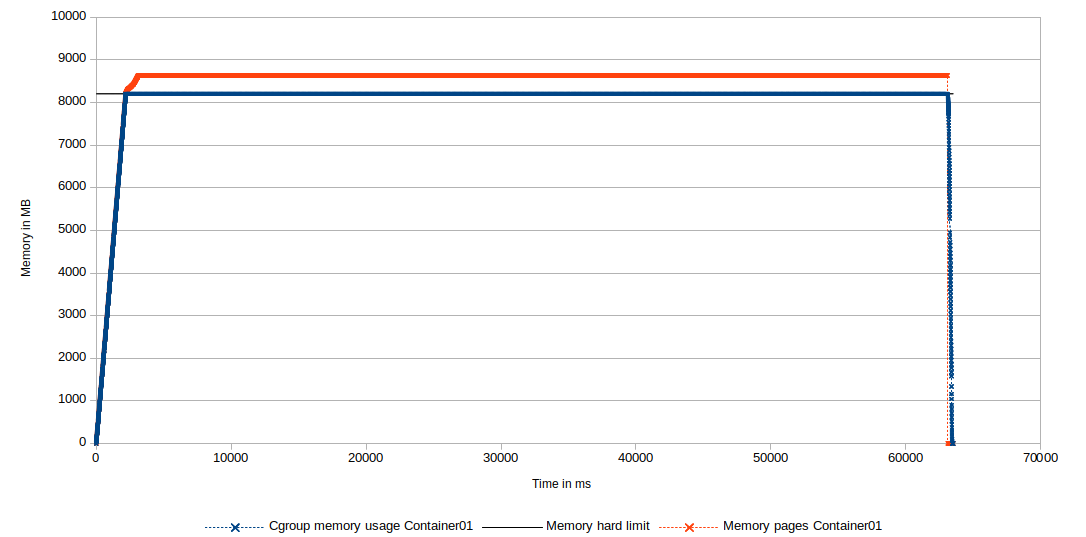
\includegraphics[width=1\linewidth]{pics/004_mem_usage_8200mb_limit_Container01_Basis_RDY_FOR_USE.png}
	\captionof{figure}[Speicher Verbrauch Cgroup 8200MB Limit]{Memory usage Cgroup 8200MB Limit}
	\label{fig:004_mem_usage_8200mb_limit_Container01_Basis_RDY_FOR_USE}
\end{minipage}

\subparagraph{Ergebnis Test04}
Wie man aus Abbildung \ref{fig:004_mem_usage_8200mb_limit_Container01_Basis_RDY_FOR_USE} entnehmen kann, ist es möglich für einen längeren Zeitraum über das Limit hinaus Ressourcen zu Allokieren. Durch die lange Ausführungszeit gleichbleibender Ressourcen ist es theoretisch möglich den Einfluss von Container untereinander zu untersuchen. Dieser Container wird von nun an als Container01 bezeichnet.

\subparagraph{Test05}
Im Ablauf des folgenden Tests wird zuerst Container01 gestartet, und während der Laufzeit wird Container02 ebenfalls eingeschaltet. Der Container02 wird zum besseren Verständnis in Abbildung \ref{fig:005_mem_usage_8200mb_limit_Container02_Basis_RDY_FOR_USE_FOCUS} nochmals in skalierter Umgebung dargestellt. 


\vspace{1em}
\begin{minipage}{\linewidth}
	\centering
	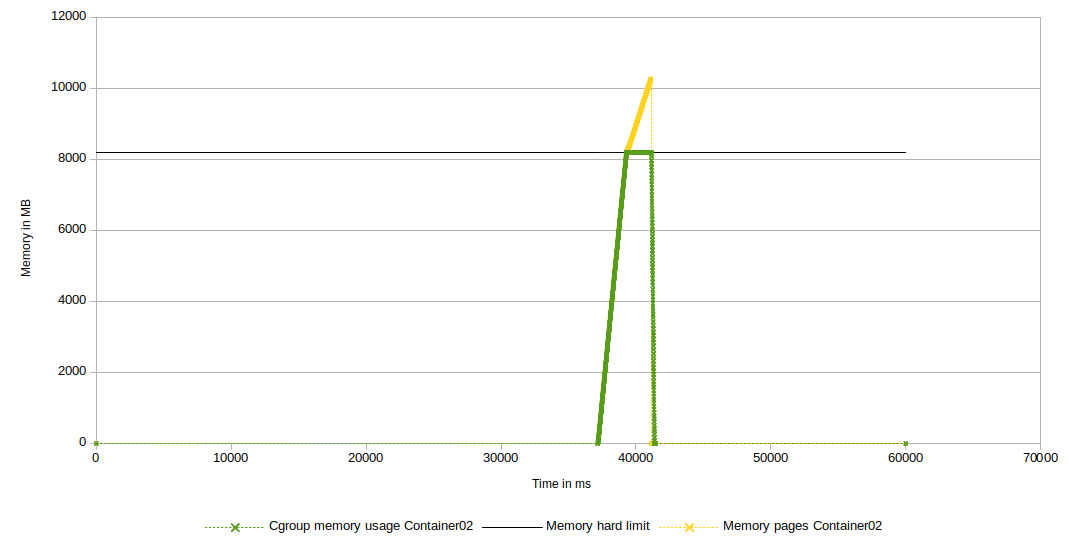
\includegraphics[width=1\linewidth]{pics/005_mem_usage_8200mb_limit_Container02_Basis_RDY_FOR_USE_FOCUS.png}
	\captionof{figure}[Speicher Verbrauch Cgroup 8200MB Limit]{Memory usage Cgroup 8200MB Limit}
	\label{fig:005_mem_usage_8200mb_limit_Container02_Basis_RDY_FOR_USE_FOCUS}
\end{minipage}

\subparagraph{Erwartungshaltung Test 05}
Die verwendbaren Systemressourcen liegen nach Abbildung \ref{fig:001_mem_usage_No_Limit_Cgroup_RDY_FOR_USE} bei etwa 14000MB. Allein Container01 verwendet schon ca. 8600MB der gesamten Summe, was die Deckelung bei Container02 auf 8200MB rein rechnerisch unnötig macht, da dieser Wert mit den verwendbaren Ressourcen nicht erreicht werden kann. 

\vspace{1em}
\begin{minipage}{\linewidth}
	\centering
	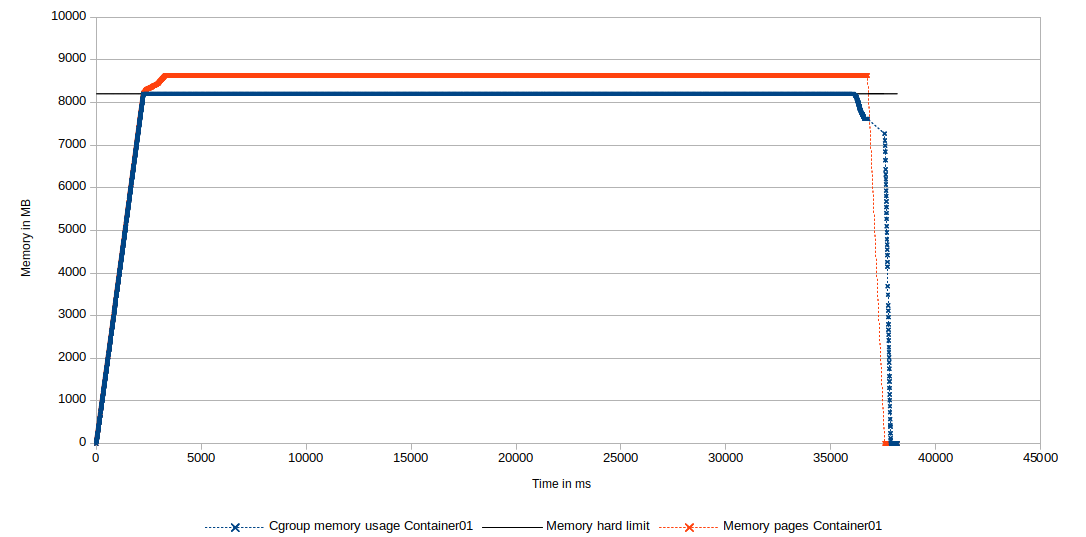
\includegraphics[width=1\linewidth]{pics/006_mem_usage_8200mb_limit_Container01_mit_ipact_RDY_FOR_USE.png}
	\captionof{figure}[Speicher Verbrauch Cgroup 8200MB Limit]{Memory usage Cgroup 8200MB Limit}
	\label{fig:006_mem_usage_8200mb_limit_Container01_mit_ipact_RDY_FOR_USE}
\end{minipage}

\subparagraph{Ergebnis Test05}
Nach Betrachtung von Abbildung \ref{fig:006_mem_usage_8200mb_limit_Container01_mit_ipact_RDY_FOR_USE} ist zu erkennen, dass Container01 nicht nach ca. 63 Sekunden geplant beendet wurde, sondern schon etwa nach ca 38 Sekunden. Was die oben genannte Hypothese nicht erfüllt.

Abbildung \ref{fig:007_mem_usage_8200mb_limit_Container01_und_Container02_RDY_FOR_USE} zeigt was passiert ist. kurz nach dem Start von Container 02 als dieser ca 5100MB Speicher Allociert hat, wird Container 01 beendet. Container 02 erreicht das Limit von 8200MB nach ca. 41 Sekunden und wird nach ca. 42,5 Sekunden ebenfalls beendet.

\vspace{1em}
\begin{minipage}{\linewidth}
	\centering
	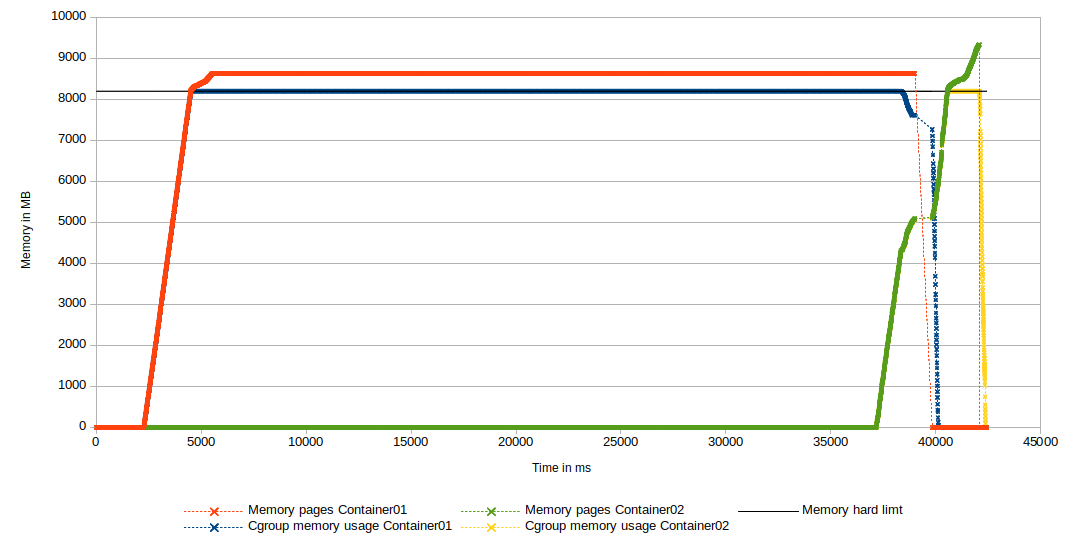
\includegraphics[width=1\linewidth]{pics/007_mem_usage_8200mb_limit_Container01_und_Container02_RDY_FOR_USE.png}
	\captionof{figure}[Speicher Verbrauch Cgroup 8200MB Limit]{Memory usage Cgroup 8200MB Limit}
	\label{fig:007_mem_usage_8200mb_limit_Container01_und_Container02_RDY_FOR_USE}
\end{minipage}

Deutlicher zu sehen ist in Abbildung \ref{fig:008_mem_usage_8200mb_limit_Container01_und_Container02_RDY_FOR_USE_FOCUS} wie die einzelnen Graphen verlaufen. 


\vspace{1em}
\begin{minipage}{\linewidth}
	\centering
	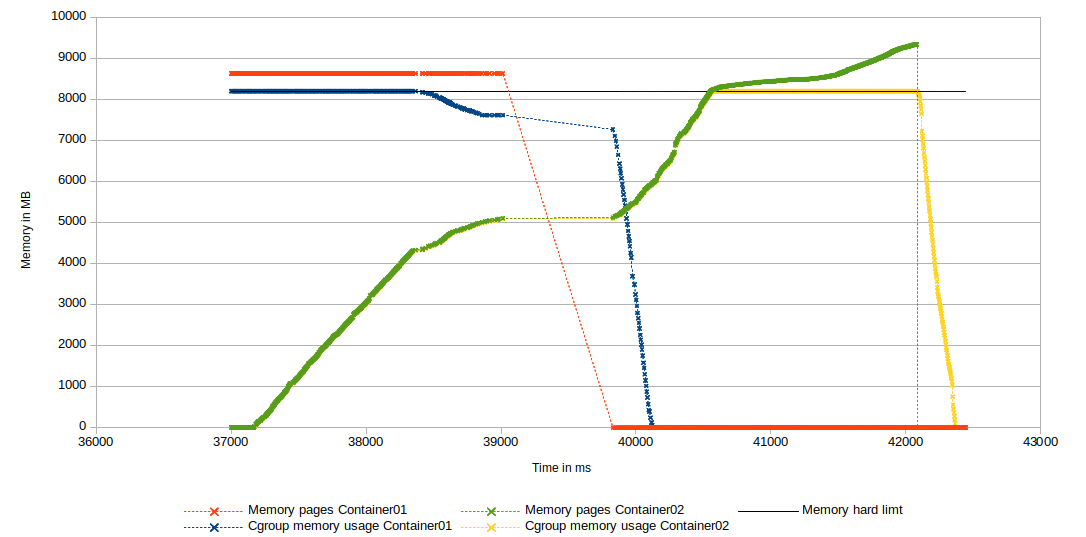
\includegraphics[width=1\linewidth]{pics/008_mem_usage_8200mb_limit_Container01_und_Container02_RDY_FOR_USE_FOCUS.png}
	\captionof{figure}[Speicher Verbrauch Cgroup 8200MB Limit]{Memory usage Cgroup 8200MB Limit}
	\label{fig:008_mem_usage_8200mb_limit_Container01_und_Container02_RDY_FOR_USE_FOCUS}
\end{minipage}

\pagebreak


% ----------------------------------------------------------------------------------
% Kapitel: Fazit und Ausblick
% ----------------------------------------------------------------------------------

%\thispagestyle{empty}
\section{Fazit und Ausblick}


Eine Kette ist nur so stark wie ihr schwächstes Glied. Ob durch einen Hacker angriff oder den Firmeninternen Administrator

Container sind konzipiert um die zur Verfügung gestellte Hardware dynamisch und dadurch effizient zu nutzen. Die Overcommitlösung im Linux-Kernel ist für die Isolation unter den Containern nicht optimal, aber für die Dynamik unerlässlich. Der große unterschied zu einer Hypervisor basierten Virtualisierungsansatz ist genau dieses Overcommitment im Ressourcen-Mangement. Während ein Hypervisor nur die Ihm zur Verfügung stehenden Ressourcen vergibt und nicht die  Ressourcen Selbst virtualisiert, sonder durch die Theoretische Teilung der Hardware mehrere Virtuelle Partitionen erstellt, besteht die Virtuallisierung des Betriebssystem-Kernels aus der Virtuellen Vergrößerung des zur Verfügung stehenden Hardwarebereichs. 

Mit den in dieser Arbeit dargestellten Gefahren von einer zu hohen Auslastung der Ressourcen ist es möglich fallstricke zu umgehen. Mit einer manuellen höheren Prioritätenvergabe im Falle eines OOM-Killer aufrufs von sicheren Containern bei denen die Images und die ausgeführten Programme überprüft wurden, sowie eine Niederwertigen Priorität für unkontrollierte und unwichtigere Container, können zumindest wichtige Prozesse geschützt werden.

Eine Möglichkeit um die Isolation zwischen den Containern zu verstärken und die Prozesse abzusichern, ist die Veränderung des Linux-Kernels. Die Kombination aus Virtueller Maschine und Container kann eine lösung in der Automobil Industrie der Zukunft sein. Je nach sicherheitsanforderung werden verschiede Over-Commit, OOM-Killer und Prioritätenvergabe Lösungen im Modifizierten Linux-Kernel implementiert, die auf einem Hypervisor mit minimalausführung eines Betriebssystems laufen. Bei Sicherheitskritischen anwendungen wie Airbag, Bremsen oder Lenkrad wird ein Linux-Kernel so umgebaut, dass die Over-Commit Variante wie bei Hypervisoren komplett herausgenommen wird und jede Anwendung seinen Eigenen Ressourcenbereich zur Verfügung gestellt bekommt und Container dadurch untereinander Stärker abgesichert sind. Bei den Blinkern oder der Innenraumlüftung kann eine Linux-Kernel Modifikation mit geringem Over-Commint ausgestattet sein und einer zusätzlichen Priorisierungsvariante im falle eines Überlaufs. Bei Anwendungen wie Innenraumbeleuchtung Autoradio oder Navigationssystem ist die ursprüngliche Over-Commitlösung implementiert um die vorhanden Ressourcen am effizientesten zu nutzen.

Aus Zeitgründen konnte in dieser Arbeit leide nicht auf alle aufgetretenen Seiteffekte eingegangen werden. 

Die Deckelung der Ressourcen durch Cgroup sollte genauer betrachtet werden. Die Tatsächliche Menge an allokiertem Speicher auf der Hardware eines Prozesses kann durch das Schreiben einer Folge von Zahlen auf den Arbeitsspeicher und das Auslesen der nachvollziebaren Speicherbereiche der Cgroup Auf der Hardware und durch das Paging verursachte verschieben der Memory Pages auf dem Massenspeicher mit der geschriebenen Folge verglichen werden. Wenn ein Teil der Zahlenvolge fehlt, ist die durch Cgroup dargestellte Partition nicht eingehalten worden. 

\pagebreak

% ----------------------------------------------------------------------------------
% Kleine Einführung in LaTeX-Elemente
% ----------------------------------------------------------------------------------

%\thispagestyle{empty}
\section{\LaTeX-Elemente}
Dieser Abschnitt beinhaltet lediglich einige Informationen über \LaTeX-Distributionen, Editoren und \LaTeX-Elemente, die Ihnen beim Einstieg in das \LaTeX-Textsatzsystem helfen sollen.

\subsection{\LaTeX-Distributionen nach Betriebssystemen}

\subsubsection{\LaTeX-Distributionen}
Folgende Haupt-\LaTeX-Distributionen stehen Ihnen zur Verfügung:
\begin{itemize}
  \item Windows:\quad \texttt{MiKTeX}\quad Webseite:\quad\url{http://www.miktex.org}
  \item Linux/Unix:\quad \texttt{TeX Live}\quad Webseite:\quad\url{http://tug.org/texlive/}
  \item Mac OS:\quad \texttt{MacTeX}\quad Webseite:\quad\url{http://www.tug.org/mactex/}
\end{itemize}

\subsubsection{\LaTeX-Editoren}
Auf folgenden Webseiten können Sie einige hilfreiche \LaTeX-Editoren finden:
\begin{itemize}
  \item Windows/Linux/Mac OS: \url{http://www.xm1math.net/texmaker/}
  \item Windiws: \url{http://www.texniccenter.org/}
  \item Mac OS: \url{http://pages.uoregon.edu/koch/texshop/}
\end{itemize}

Falls bei den oben genannten Editoren kein passender vorhanden war, findet sich auf Wikipedia eine Zusammenstellung vieler weiterer \LaTeX-Editoren:\\[1em]
\hspace*{3cm}\url{https://en.wikipedia.org/wiki/Comparison_of_TeX_editors}


\subsection{Bilder}
Zum Einfügen eines Bildes, siehe Abbildung \ref{fig:reversi01}, werden die \texttt{minipage}-Umgebung und der Befehl \texttt{$\backslash$includegraphics} genutzt, da die Bilder so gut positioniert und einfach integriert und skaliert werden können.

\vspace{1em}
\begin{minipage}{\linewidth}
	\centering
	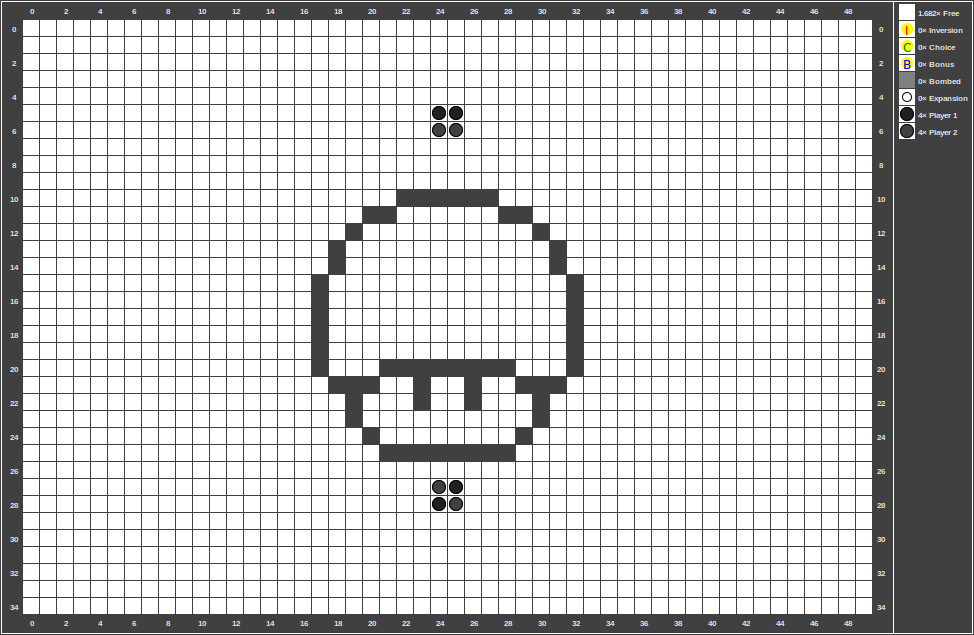
\includegraphics[width=0.5\linewidth]{pics/gamefield01.png}
	\captionof{figure}[Spielfeld 01]{Unbespieltes Spielfeld\footnotemark }
	\label{fig:reversi01}
\end{minipage}
\footnotetext{Diesem Spielfeld wurden noch keine Spieler zugewiesen (daher die dunklen Spielsteine)}

Nachdem das Spielt gestartet wurde und beide Spielphasen durchlaufen wurden, siegt schließlich der Spieler mit der Farbe rot.

%\vspace{1em}
%\begin{minipage}{\linewidth}
%	\centering
%	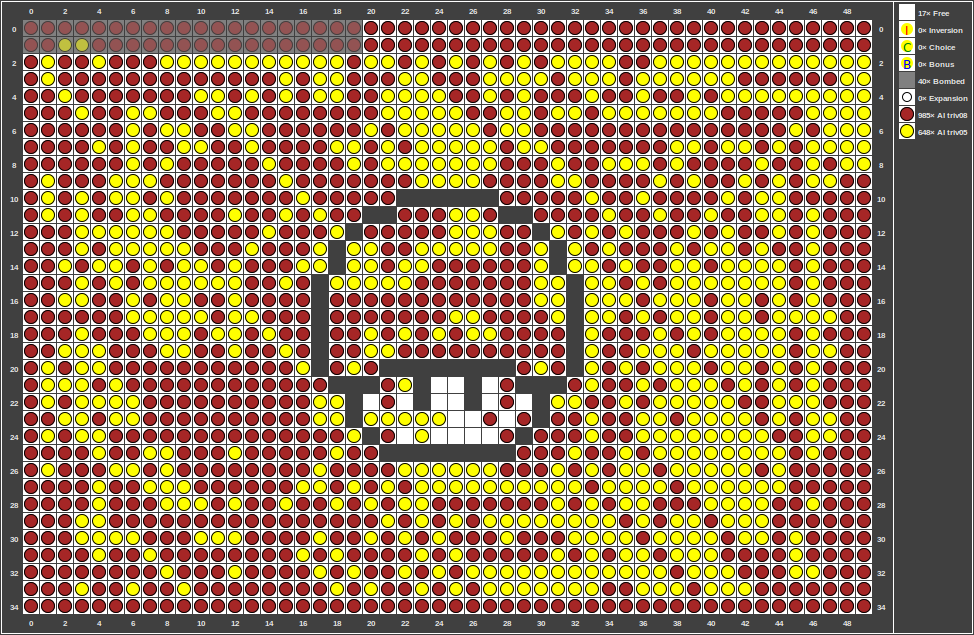
\includegraphics[width=0.5\linewidth]{pics/gamefield02.png}
%	\captionof{figure}[Spielfeld 02]{Finales Spielfeld\footnotemark }
%	\label{fig:reversi2}
%\end{minipage}
%\footnotetext{Das Spielfeld nach der Zug- und Bombenphase. Spieler rot gewinnt eindeutig.}

\subsection{Tabellen}
In diesem Abschnitt wird eine Tabelle (siehe Tabelle \ref{tab:beispiel}) dargestellt.

\vspace{1em}
\begin{table}[!h]
	\centering
	\begin{tabular}{|l|l|l|}
		\hline
		\textbf{Name} & \textbf{Name} & \textbf{Name}\\
		\hline
		1 & 2 & 3\\
		\hline
		4 & 5 & 6\\
		\hline
		7 & 8 & 9\\
		\hline
	\end{tabular}
	\caption{Beispieltabelle}
	\label{tab:beispiel}
\end{table}


\subsection{Auflistung}
Für Auflistungen wird die \texttt{enumerate}- oder \texttt{itemize}-Umgebung genutzt.

\begin{itemize}
	\item Nur
	\item ein
	\item Beispiel.
\end{itemize}

\subsection{Listings}
Zuletzt sehen Sie in Listing \ref{lst:maxTeilsumZweiD} ein Beispiel für das Einbinden von Quellcode mit Syntax-Highlighting.

\vspace{1em}
\lstinputlisting[caption=Brute Force-Ansatz für das MaxTeilsum2D-Problem, label=lst:maxTeilsumZweiD,basicstyle=\ttfamily\scriptsize]{code/maxTeilsum2DBruteForce.txt}

\subsection{Selbstgestaltete Abbildungen}
Mithilfe des Paketes \texttt{tikz} können sehr schöne Abbildungen (z.\,B.\ Automaten, Graphen etc.) direkt in \LaTeX generiert werden. Viele Beispiele dazu finden Sie auf folgender Webseite:\\[1em]
\hspace*{3cm}\url{http://www.texample.net/tikz/}.

\subsection{Tipps}
Die Literaturreferenzen (Bücher, Paper und Journals) und Internetquellen (Webseiten, Blogs etc.) befinden sich in der Datei \textit{literatur.bib}. Eine Buch- und eine Online-Quelle sind beispielhaft eingefügt.  %\cite{Bui2015AnalysisSecurity} 

Literatur und Quellen werden in zwei getrennte Verzeichnisse aufgeteilt. Als Unterscheidungsmerkmal dient bei den Quellen der Zusatz: \texttt{keywords = \{online\}}.

\pagebreak

% ----------------------------------------------------------------------------------------------------------
% Filter fuer Literatur und Quellen definieren
% ----------------------------------------------------------------------------------------------------------

%\defbibheading{Literatur}{\section*{Literaturverzeichnis}} 
\defbibheading{Quellen}{\section*{Quellenverzeichnis}} 
  
%\defbibfilter{Literatur}{\not\keyword{online}} 
%\defbibfilter{Quellen}{\keyword{online}} 


% ----------------------------------------------------------------------------------------------------------
% Literatur
% ----------------------------------------------------------------------------------------------------------
%\lhead{} 
%\rhead{Literaturverzeichnis} 

%\printbibliography[heading=Literatur,filter=Literatur] 

%\pagebreak


% ---------------------------------------------------------------------------------------------------------- 
% Quellen 
% ---------------------------------------------------------------------------------------------------------- 
\lhead{} 
\rhead{Quellenverzeichnis} 

%\printbibliography[title = {Quellenverzeichnis}, heading=Quellen] 
%\printbibliography[title = {Quellenverzeichnis},
\printbibliography[title = {Quellenverzeichnis}, heading=Quellen]

\pagebreak 

% ----------------------------------------------------------------------------------------------------------
% Anhang
% ----------------------------------------------------------------------------------------------------------
\pagenumbering{Roman}
\setcounter{page}{1}
\lhead{Anhang \thesection}

\begin{appendix}
\section*{Anhang}
\phantomsection
\addcontentsline{toc}{section}{Anhang}
\addtocontents{toc}{\vspace{-0.5em}}

Inhalt des beigefügten Datenträgers:
\begin{itemize}
  \item $\ldots$
  \item $\ldots$
\end{itemize}

\section{Domändenmodell}
Ein toller Anhang, der nicht nur als \glqq{}\emph{Müllhalde}\grqq{} genutzt wird, sondern in dem Bilder und Inhalte auch mit eigenen Worten erklärt werden und den man auch für sich alleine lesen kann. Es sollten auch Referenzen auf die zugehörige ausführliche Behandlung im Hauptteil inklusive Seitenangabe mit $\backslash$\texttt{pageref} gegeben werden.

\subsection*{Screenshot}
\label{app:screenshot}
Unterkategorie, die nicht im Inhaltsverzeichnis auftaucht.

\end{appendix}


\pagebreak


%\bibliographystyle{ieeetr}
%\bibliography{mendeley}
\end{document}

